\section{\textbf{Introduction}}

The Transformer was introduced as a complete encoder--decoder architecture for sequence transduction \cite{vaswani2017attention}. Its encoder constructs contextual representations of an input sequence, while its decoder combines a causal output state with encoder information to generate a conditional sequence. Subsequent progress has produced highly capable but increasingly specialized families. Encoder-oriented models such as BERT emphasize bidirectional representation learning \cite{devlin2019bert}; Vision Transformers apply encoder-style processing to image patches \cite{dosovitskiy2021image}; and GPT-style models emphasize causal decoder stacks for autoregressive generation \cite{brown2020language}. These specializations have been productive, but they divide perception, representation, and generation across model families that are not inherently organized as one persistent agent.

Multimodal research has begun to reconnect these capabilities. Flamingo conditions a language model on visual representations through gated cross-attention \cite{alayrac2022flamingo}; PaLM-E injects continuous sensor representations into an embodied language model \cite{driess2023palme}; Perceiver IO maps heterogeneous inputs and outputs through a shared latent space \cite{jaegle2022perceiver}; and Gato represents multiple modalities, tasks, embodiments, and action spaces as token sequences processed by one generalist policy \cite{reed2022generalist}. These systems demonstrate that heterogeneous observations and outputs can participate in shared computation. Nevertheless, processing several modalities is not by itself equivalent to an architecture in which multimodal perception, internal thought, and action continuously condition one another.

Commercial AI platforms now reinforce this distinction. Systems such as ChatGPT and Claude expose broad conversational interfaces through which users can analyze text, images, and documents and invoke additional tools or services \cite{openai2026chatgpt,anthropic2026claude}. From the user's perspective, these systems can resemble integrated intelligence because heterogeneous requests enter through one interface and useful responses or actions return through the same interface. However, an end-to-end service is not necessarily an end-to-end neural architecture. Public interfaces do not reveal the complete internal architectures of proprietary systems, and this paper therefore makes no claim about their undisclosed implementations. What can be observed more generally is a system-level design pattern in which language models coordinate modality-specific models, retrieval components, tools, and execution environments. HuggingGPT provides a published example: a language model plans a task, selects expert models, executes the selected models, and summarizes their outputs across language, vision, and speech tasks \cite{shen2023hugginggpt}.

This orchestration pattern is powerful and immediately practical, but it introduces a distinction among three levels of integration. \textit{Interface integration} presents multiple capabilities through one interaction surface. \textit{System integration} connects models and tools through software, routing rules, intermediate representations, and execution logic. \textit{Architectural integration} learns the relationships among perception, internal state, and action within a jointly trainable neural architecture. The first two levels can provide broad functionality, yet architectures of this class may require model selection, data conversion, prompt construction, communication among components, and separate deployment and maintenance paths. These operations can add engineering complexity, latency, and computational overhead. They can also prevent errors originating in an early specialist or textual conversion from being corrected through direct end-to-end learning. This observation does not diminish modular systems; it motivates a complementary question: can more of the integration currently achieved by external orchestration be learned within one architecture?

Our preceding work provides the conceptual path to this question. Intelligence was defined operationally as information-dependent selection among possible actions, states, or outputs, while remaining distinct from phenomenal consciousness \cite{zohourian2026intelligence}. Artificial consciousness was then considered in multiple possible forms, with language proposed as a unifying interface through which heterogeneous artificial minds can communicate without requiring identical internal representations \cite{zohourian2026language}. We subsequently distinguished artificial general intelligence from consciousness and characterized AGI as integrated multimodal agency: the coordination of perception, memory, objectives, reasoning, planning, and action across modalities, tasks, and environments \cite{zohourian2026agi}. Finally, we separated general intelligence from superintelligence, defining the latter through machine capabilities that extend the frontier of knowledge by discovery, fusion, or invention rather than merely reproducing or accelerating known procedures \cite{zohourian2026superintelligence}. Together, these arguments identify integrated agency as an architectural problem that precedes claims of either consciousness or superintelligence.

This paper introduces \textit{AGI-Former}, a novel and testable end-to-end deep learning architecture designed to support artificial general intelligence as integrated multimodal agency. AGI-Former directly connects modality-specific perception encoders with causal thought and action generation. Image, video, audio, language, and additional sensory streams are encoded in forms appropriate to their native structure; a decoder state formed from prior thought and action tokens then queries and combines the encoded evidence to generate subsequent thought or action tokens. In this end-to-end mapping, multimodal observations and prior thought or action tokens jointly condition the next thought or action tokens.

The phrase \textit{architecture for AGI} is used deliberately but conservatively. AGI-Former is intended to operationalize the architectural requirements of integrated multimodal agency; it does not imply that any untrained instantiation is generally intelligent, that multimodality alone is sufficient for AGI, or that the architecture establishes consciousness. Its claim is instead scientific and falsifiable: the proposed organization can be implemented, trained, ablated, and compared against modular and partially integrated alternatives using measurable perception, reasoning, coordination, transfer, and action outcomes.

AGI-Former includes an evolutionary baseline as well as the proposed joint architecture. In the baseline organization, image--text, video--text, audio--text, and other modality-to-language specialists convert observations into descriptions that are supplied to a large language model supervisor. The supervisor integrates these descriptions and produces plans, tool calls, or actions. This disjoint organization is compatible with existing components and demonstrates the value of language as an interoperability layer. However, it also makes explicit the limitations of text-mediated integration: modality-native detail can be compressed before joint reasoning begins, specialist errors can propagate forward, and perception cannot be optimized directly against the final action unless gradients and training signals cross the complete pipeline.

The joint AGI-Former architecture removes this required textual bottleneck. Modality-specific encoders preserve the structure of each sensory stream while making their encoded representations directly available to a shared decoder-side thought--action state. The decoder does not merely receive descriptions of observations; it learns which portions of each encoded stream are relevant to the current state and how the selected evidence should affect the next decision. This organization follows the broader principle that multimodal learning depends not only on representation but also on when and how information is aligned and fused \cite{baltrusaitis2019multimodal}.

AGI-Former builds technically upon Unified Attention for Image Classification and Captioning (UTR) \cite{zohourian2026utr}. UTR treats encoding and conditional generation as related attention problems and develops unified attention operations for interactions within and between information streams. AGI-Former extends this foundation from vision--language learning to multimodal agency. The essential transition is from mapping an encoded modality to a descriptive sequence toward mapping several encoded modalities and an evolving causal state to thoughts and actions capable of affecting an environment.

Figure~\ref{fig:transformer_transition} motivates this transition. Rather than treating encoder-only and decoder-only Transformer families as unrelated endpoints, AGI-Former returns to the complete encoder--decoder relation as the fundamental computational unit. Encoders construct representations of what the agent observes; decoder tokens represent what the agent has thought or done; and cross-attention determines which encoded information should condition what the agent thinks or does next. Modality-specific tokenization remains necessary, but the relationship between perception and action is shared and jointly trainable.

\begin{figure*}[t]
    \centering
    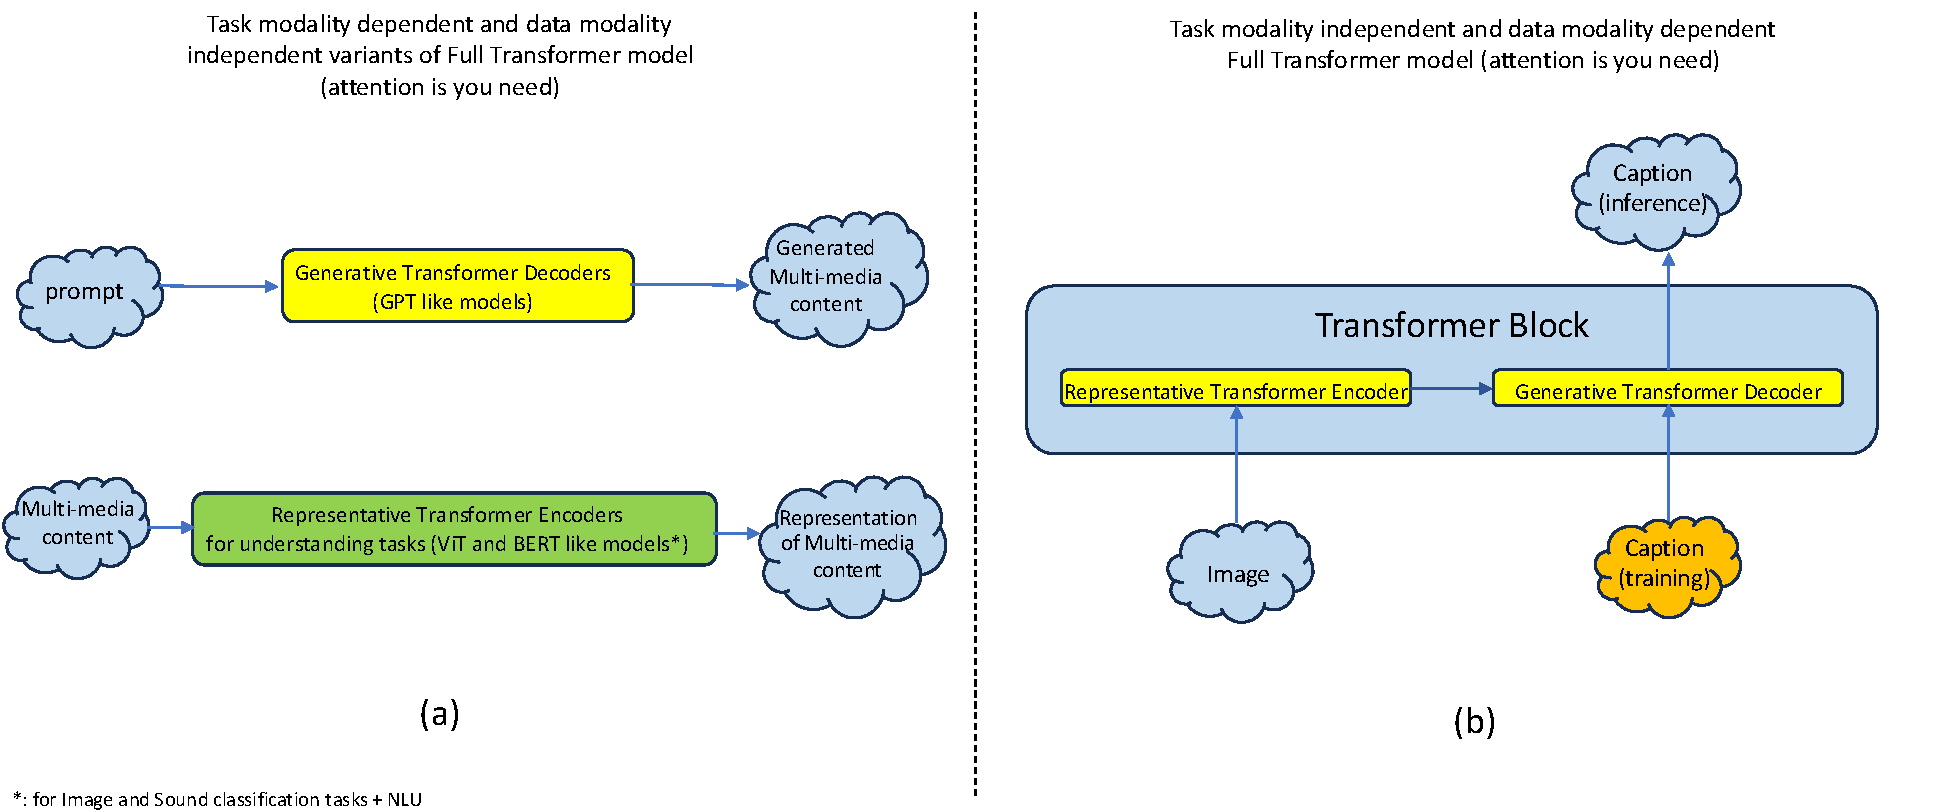
\includegraphics[width=\textwidth]{Figures/fig1.pdf}
    \caption{Conceptual transition from specialized Transformer components to a complete encoder--decoder organization for multimodal perception and conditional thought or action generation.}
    \label{fig:transformer_transition}
\end{figure*}

The proposed framework contains two complementary output organizations. The first generates disjoint modality-conditioned action-token streams. A shared causal thought--action state attends to each encoded modality independently, preserving distinct output spaces or execution requirements when a task demands them. The second generates a joint action-token stream. Each modality is first conditioned on the current thought--action state; the resulting task-relevant representations are then concatenated and used to synthesize one coordinated output. This ordering implements action-conditioned late fusion: the architecture selects relevant evidence within each modality before integrating that evidence into a common decision.

The central hypothesis of AGI-Former is that artificial general intelligence requires more than access to several modalities or the appearance of integration at an interface. It requires an end-to-end trainable mechanism through which multimodal perception, internal thought, and action can repeatedly condition one another. The principal contributions of this paper are as follows:

\begin{itemize}
    \item We introduce AGI-Former as a testable end-to-end encoder--decoder architecture for integrating multimodal perception with causal thought and action generation.
    \item We distinguish interface-level and system-level integration from architectural integration, positioning existing model-and-tool orchestration as a practical baseline rather than the endpoint of multimodal agency.
    \item We define a disjoint specialist organization in which modality-to-language systems communicate with a language-model supervisor, providing an implementable comparison architecture and an evolutionary path toward joint learning.
    \item We propose modality-specific encoders coupled to a shared decoder-side thought--action state, allowing modality-native evidence to participate directly in conditional generation.
    \item We formulate complementary disjoint-output and joint-output organizations, including action-conditioned late fusion for coordinated multimodal decisions.
    \item We extend the unified-attention direction introduced in UTR from image classification and captioning toward multimodal perception, reasoning, and agency, and define a falsifiable experimental program based on training, ablation, transfer, coordination, and action performance.
\end{itemize}

The remainder of this paper reviews the relevant Transformer, multimodal, and generalist-agent literature; formalizes the input representations and unified attention operations; presents the disjoint and joint AGI-Former architectures; specifies training objectives and evaluation protocols; and concludes with limitations and directions for implementation.
